% !TEX program = xelatex
% =====================================================================
%  Generated by figrepro -- do not edit by hand, edit the Figure spec.
%  Source canvas: 5811 x 3837 px   ->   170.00 mm wide
%  Compile with xelatex (fontspec is required).
% =====================================================================
\documentclass[tikz,border=0pt]{standalone}
\usepackage{fontspec}
\setmainfont{Times New Roman}
\usepackage{graphicx}
\usepackage{tikz}
\usetikzlibrary{calc}
\definecolor{greenF}{HTML}{F0F8EB}
\definecolor{greenB}{HTML}{C9E5B4}
\definecolor{creamF}{HTML}{FEF7F1}
\definecolor{creamB}{HTML}{FCE7D6}
\definecolor{cyanF}{HTML}{EAF9F9}
\definecolor{cyanB}{HTML}{D4F4F1}
\definecolor{orangF}{HTML}{EF822F}
\definecolor{greenA}{HTML}{75BC42}
\definecolor{c8}{HTML}{F0F8EB}
\definecolor{c9}{HTML}{C9E5B4}
\definecolor{c10}{HTML}{FEF7F1}
\definecolor{c11}{HTML}{FCE7D6}
\definecolor{c13}{HTML}{EAF9F9}
\definecolor{c14}{HTML}{D4F4F1}
\definecolor{c15}{HTML}{75BC42}
\definecolor{c16}{HTML}{EF822F}
\tikzset{fdash0/.style={dash pattern=on 3.8976pt off 3.1512pt}}
\begin{document}
\begin{tikzpicture}[x=0.029255mm, y=-0.029255mm, line cap=butt, line join=miter,
                   every node/.style={inner sep=0pt, outer sep=0pt}]
\draw[fill=c8, draw=black, line width=0.99513pt, rounded corners=3.1888mm] (40,196) rectangle (1543,1667);
\draw[fill=c8, draw=black, line width=0.66342pt, rounded corners=1.9308mm] (118,421) rectangle (684,1614);
\draw[fill=c8, draw=black, line width=0.66342pt, rounded corners=1.9308mm] (872,421) rectangle (1439,1614);
\draw[fill=c9, draw=black, line width=0.99513pt, rounded corners=0.23404mm, fdash0] (196,481) rectangle (623,646);
\draw[fill=c9, draw=black, line width=0.99513pt, rounded corners=0.23404mm, fdash0] (196,699) rectangle (623,864);
\draw[fill=c9, draw=black, line width=0.99513pt, rounded corners=0.23404mm, fdash0] (196,916) rectangle (623,1081);
\draw[fill=c9, draw=black, line width=0.99513pt, rounded corners=0.23404mm, fdash0] (196,1133) rectangle (623,1298);
\draw[fill=c9, draw=black, line width=0.99513pt, rounded corners=0.23404mm, fdash0] (196,1363) rectangle (623,1528);
\draw[fill=c9, draw=black, line width=0.99513pt, rounded corners=0.23404mm, fdash0] (950,475) rectangle (1377,640);
\draw[fill=c9, draw=black, line width=0.99513pt, rounded corners=0.23404mm, fdash0] (950,769) rectangle (1377,934);
\draw[fill=c9, draw=black, line width=0.99513pt, rounded corners=0.23404mm, fdash0] (950,1064) rectangle (1377,1229);
\draw[fill=c9, draw=black, line width=0.99513pt, rounded corners=0.23404mm, fdash0] (950,1358) rectangle (1377,1523);
\draw[fill=c10, draw=black, line width=0.99513pt, rounded corners=3.1888mm] (1957,201) rectangle (5772,1672);
\draw[fill=c11, draw=black, line width=0.99513pt, rounded corners=0.23404mm, fdash0] (2037,365) rectangle (2663,580);
\draw[fill=c11, draw=black, line width=0.99513pt, rounded corners=0.23404mm, fdash0] (2037,820) rectangle (2663,1035);
\draw[fill=c11, draw=black, line width=0.99513pt, rounded corners=0.23404mm, fdash0] (2037,1275) rectangle (2663,1490);
\draw[fill=white, draw=black, line width=0.99513pt] (3064,241) rectangle (4321,1177);
\draw[fill=white, draw=black, line width=0.99513pt] (4390,241) rectangle (5648,1177);
\draw[fill=c11, draw=black, line width=0.99513pt, rounded corners=0.23404mm, fdash0] (3325,1357) rectangle (5385,1608);
\draw[fill=c13, draw=black, line width=0.99513pt, rounded corners=3.8616mm] (40,2091) rectangle (5772,3813);
\draw[fill=white, draw=black, line width=0.99513pt] (181,2402) rectangle (1642,3624);
\draw[fill=none, draw=black, line width=0.99513pt] (1802,2402) rectangle (3852,3624);
\draw[fill=white, draw=black, line width=0.99513pt] (3992,2402) rectangle (5647,3624);
\draw[fill=c14, draw=black, line width=0.99513pt, rounded corners=0.23404mm, fdash0] (2355,2482) rectangle (3291,2697);
\draw[fill=c14, draw=black, line width=0.99513pt, rounded corners=0.23404mm, fdash0] (2255,2817) rectangle (3398,3117);
\draw[fill=c14, draw=black, line width=0.99513pt, rounded corners=0.23404mm, fdash0] (1873,3235) rectangle (2755,3535);
\draw[fill=c14, draw=black, line width=0.99513pt, rounded corners=0.23404mm, fdash0] (2865,3235) rectangle (3747,3535);
\node at (3692,709) {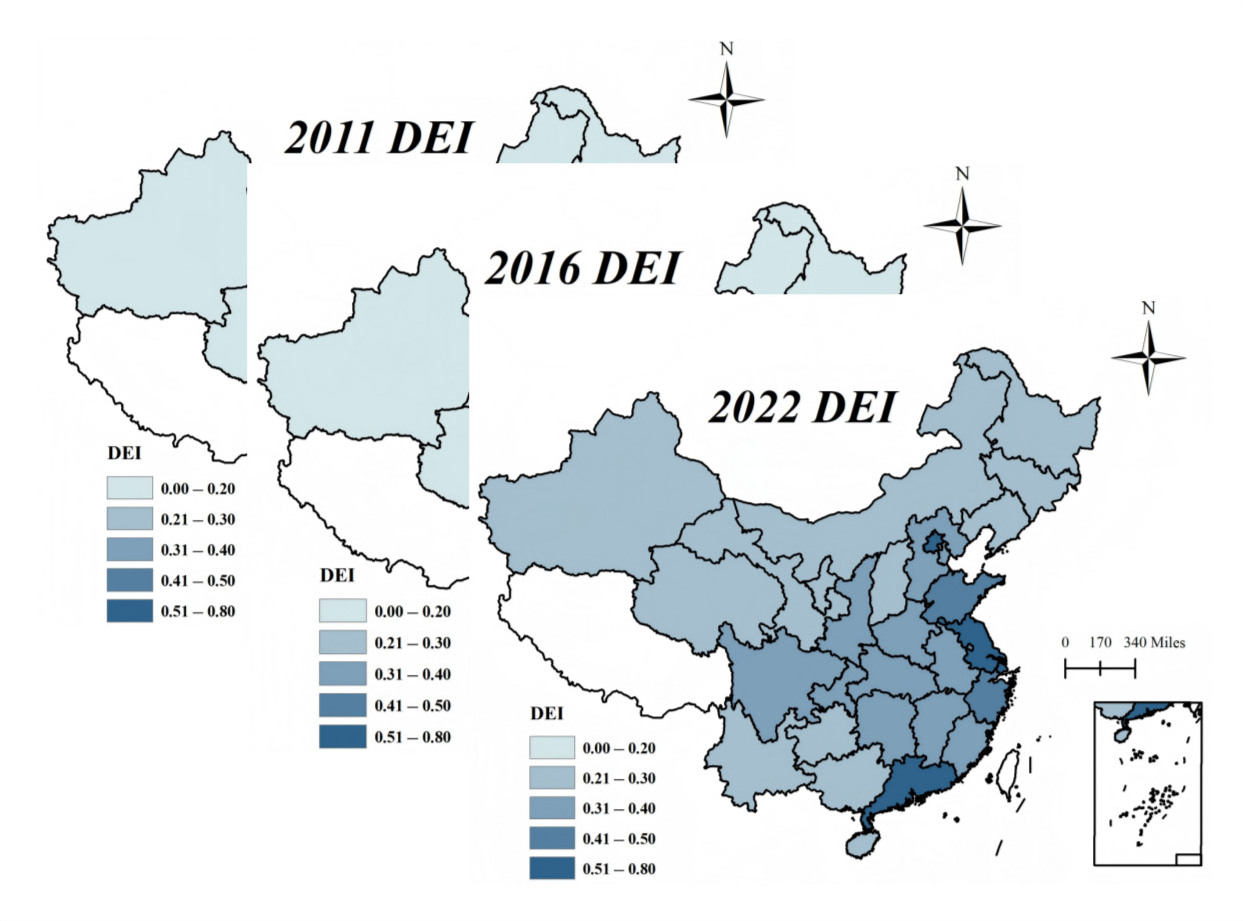
\includegraphics[width=36.42mm,height=27.03mm]{panel_dei_maps.png}};
\node at (5019,709) {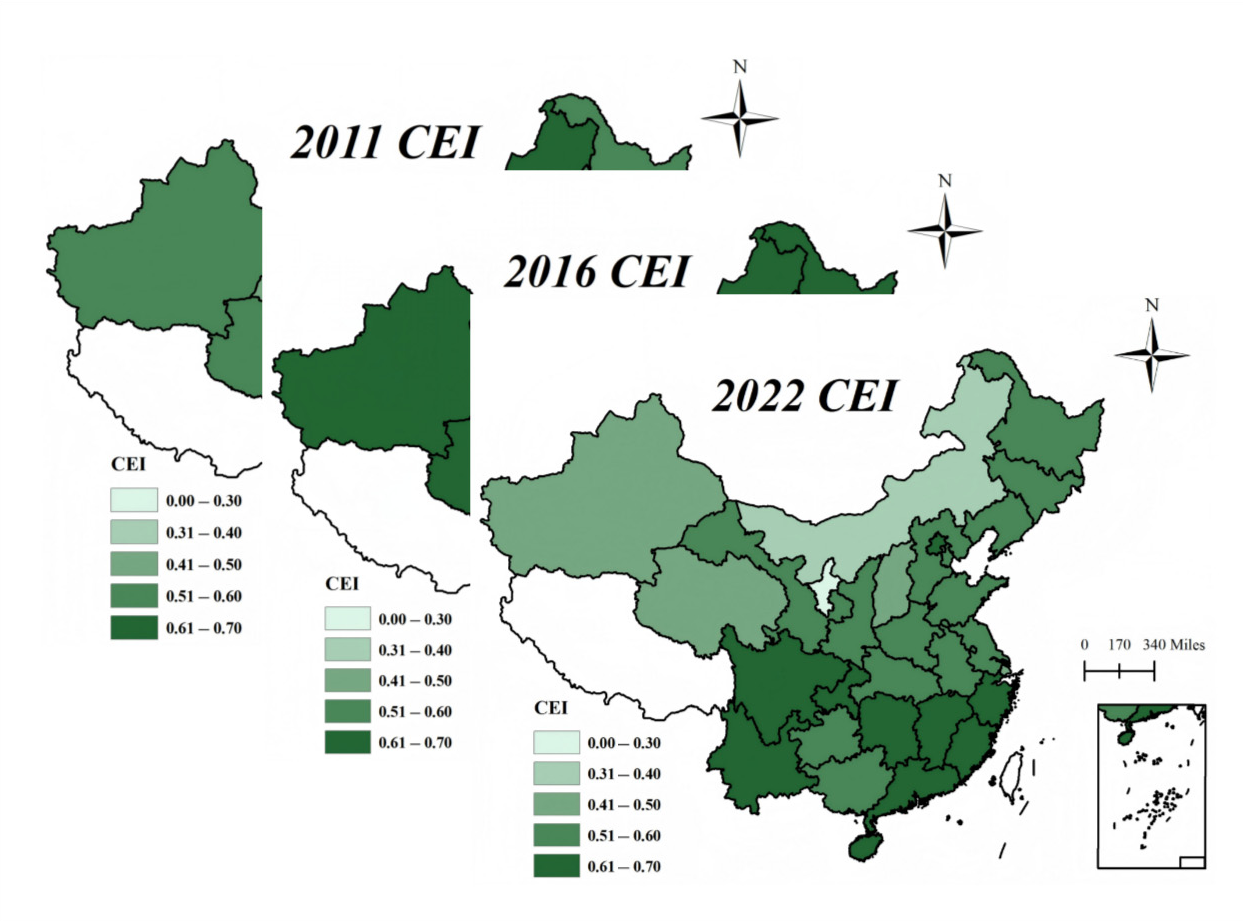
\includegraphics[width=36.45mm,height=27.03mm]{panel_cei_maps.png}};
\node at (911.5,3013) {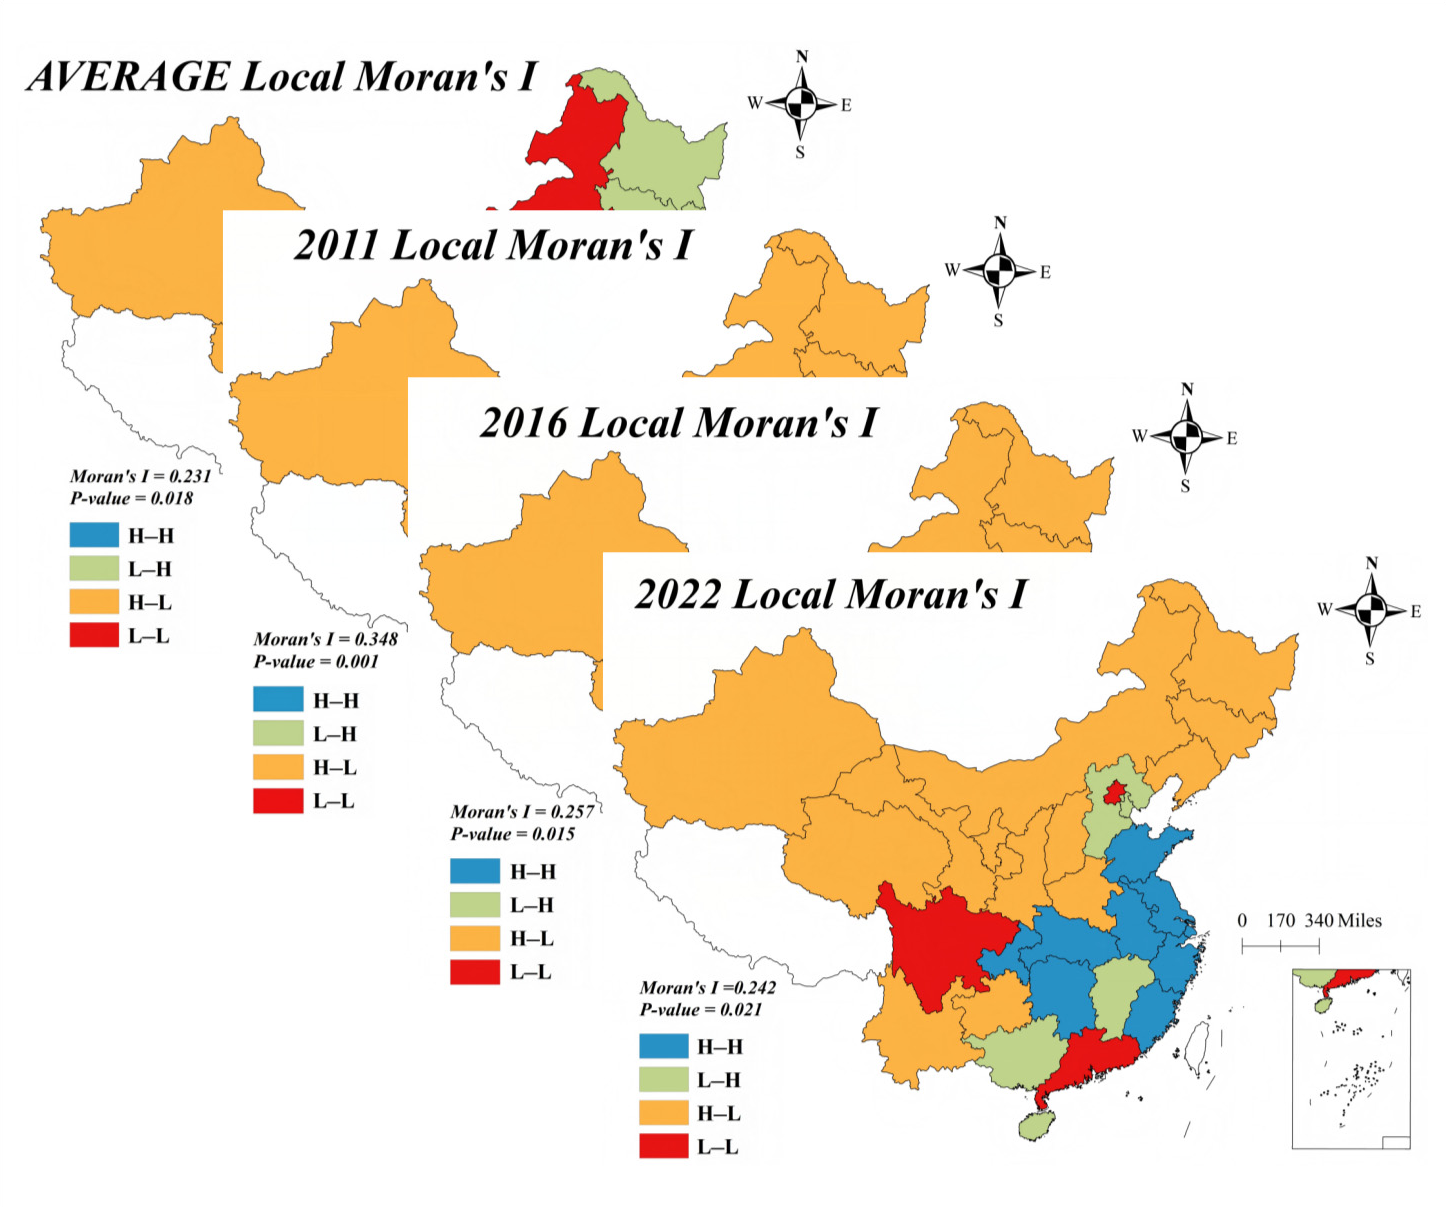
\includegraphics[width=42.39mm,height=35.4mm]{panel_moran_map.png}};
\node at (4820,3013) {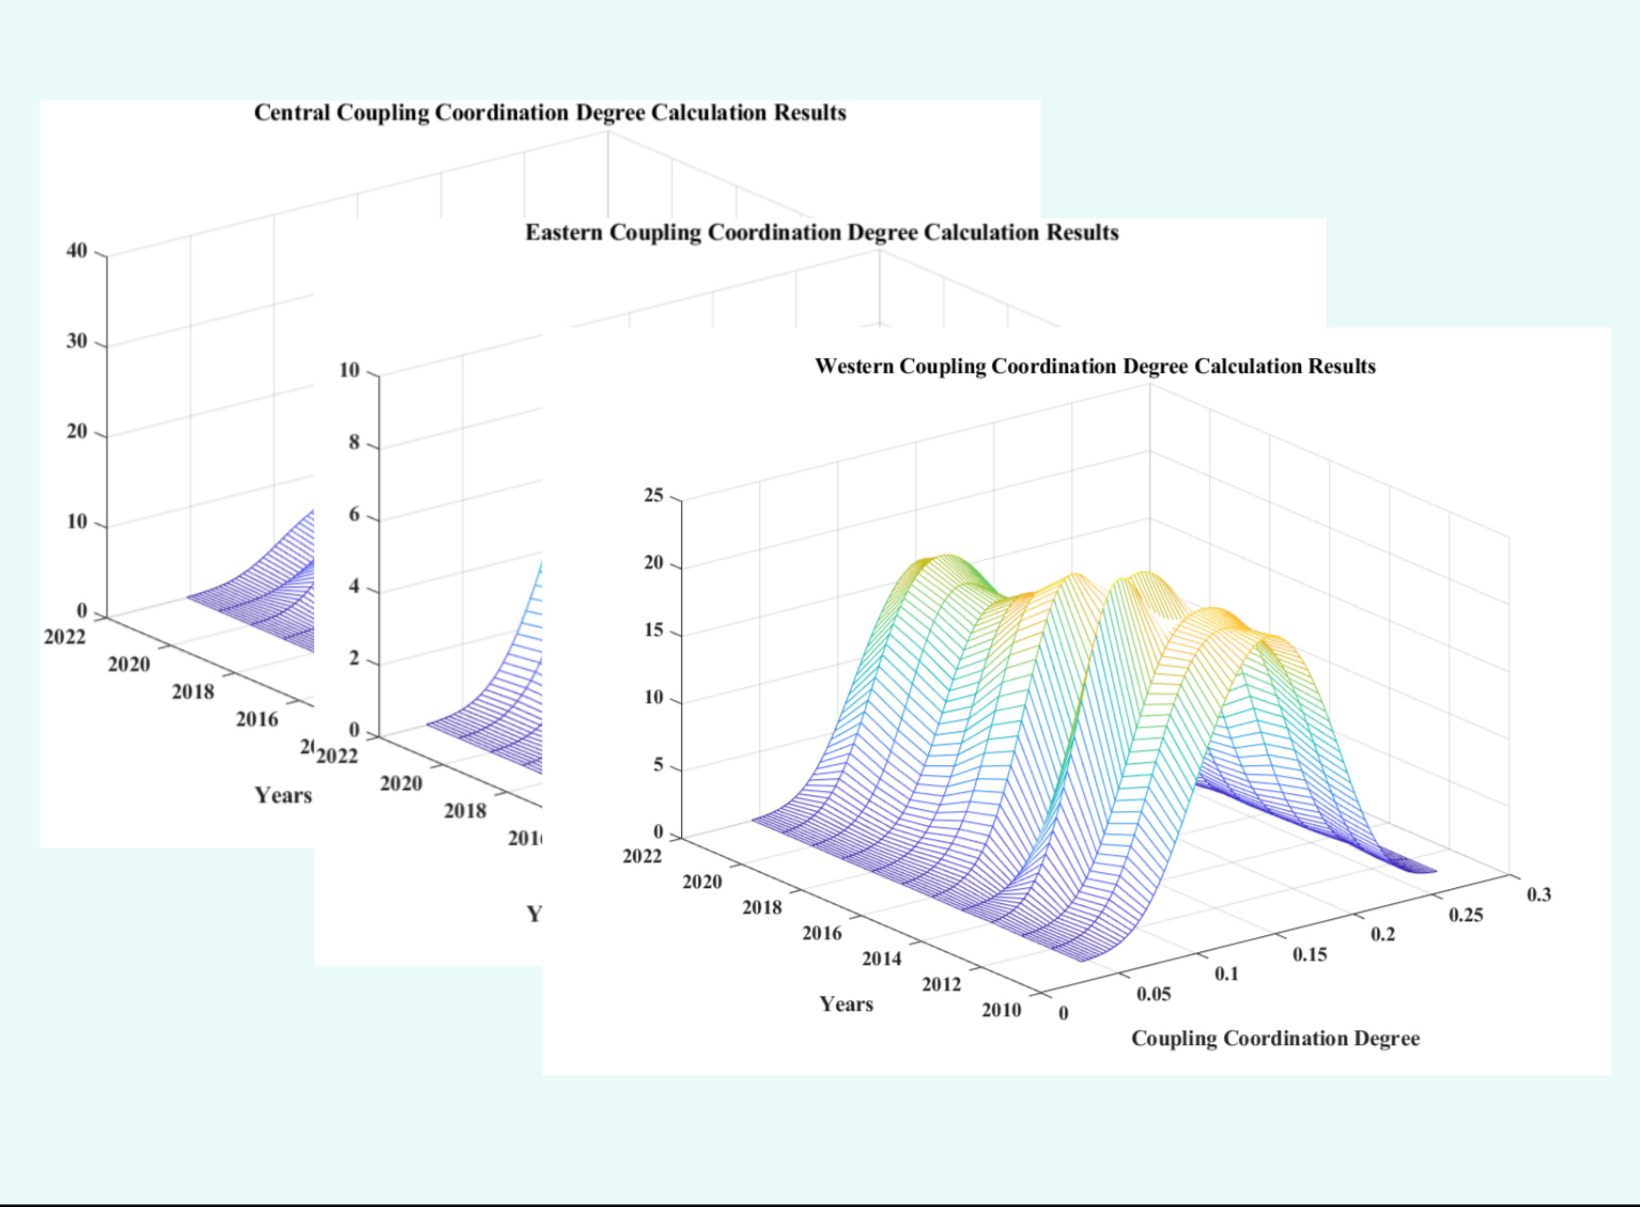
\includegraphics[width=48.07mm,height=35.4mm]{panel_kde_3d.png}};
\draw[fill=c15, draw=black, line width=0.70488pt] (1605,885) -- (1770,885) -- (1770,833) -- (1865,932) -- (1770,1031) -- (1770,977) -- (1605,977) -- cycle;
\draw[line width=0.66342pt] (2805,458) .. controls (2806,458) and (2832,513) .. (2832,608) -- (2832,777.3) .. controls (2832,901.5) and (2844,927.5) .. (2900,927.5) .. controls (2844,927.5) and (2832,953.5) .. (2832,1078) -- (2832,1247) .. controls (2832,1342) and (2806,1397) .. (2805,1397);
\draw[line width=0.66342pt] (2897,926) -- (2982,926);
\draw[line width=0.66342pt] (3692,1183) -- (3692,1266) -- (5018,1266) -- (5018,1183);
\draw[line width=0.66342pt] (4354,1266) -- (4354,1313);
\fill (4332,1311) -- (4376,1311) -- (4354,1351) -- cycle;
\draw[fill=c16, draw=black, line width=0.66342pt] (2851,1750) -- (2942,1750) -- (2942,1929) -- (2977,1929) -- (2896,2002) -- (2816,1929) -- (2851,1929) -- cycle;
\draw[fill=c16, draw=black, line width=0.66342pt] (3853,1750) -- (3944,1750) -- (3944,1929) -- (3979,1929) -- (3898,2002) -- (3818,1929) -- (3853,1929) -- cycle;
\draw[fill=c16, draw=black, line width=0.66342pt] (4854,1750) -- (4944,1750) -- (4944,1929) -- (4980,1929) -- (4899,2002) -- (4818,1929) -- (4854,1929) -- cycle;
\draw[line width=0.66342pt] (2824,2703) -- (2824,2773);
\fill (2802,2771) -- (2846,2771) -- (2824,2811) -- cycle;
\draw[line width=0.66342pt] (2826,3123) -- (2826,3175);
\draw[line width=0.66342pt] (2314,3175) -- (3306,3175);
\draw[line width=0.66342pt] (2314,3175) -- (2314,3189);
\fill (2293,3187) -- (2335,3187) -- (2314,3229) -- cycle;
\draw[line width=0.66342pt] (3306,3175) -- (3306,3189);
\fill (3285,3187) -- (3327,3187) -- (3306,3229) -- cycle;
\node[anchor=base west] at (150,128) {\fontsize{13.3pt}{15.3pt}\selectfont \bfseries Indicator Selection};
\node[anchor=base west] at (2018,130) {\fontsize{13.3pt}{15.3pt}\selectfont \bfseries Measurement Model};
\node[anchor=base] at (403.5,359) {\fontsize{11.8pt}{13.6pt}\selectfont \bfseries\itshape DEI};
\node[anchor=base] at (1165,361) {\fontsize{11.8pt}{13.6pt}\selectfont \bfseries\itshape CEI};
\node[anchor=base] at (409,590) {\fontsize{6.77pt}{7.78pt}\selectfont \bfseries Domains};
\node[anchor=base] at (409,808) {\fontsize{6.77pt}{7.78pt}\selectfont \bfseries IPv4};
\node[anchor=base] at (409,1025) {\fontsize{6.77pt}{7.78pt}\selectfont \bfseries IAP};
\node[anchor=base] at (409,1472) {\fontsize{6.77pt}{7.78pt}\selectfont \bfseries DFFD};
\fill (372.5,1235) circle (0.3364mm);
\fill (408.5,1235) circle (0.3364mm);
\fill (444.5,1235) circle (0.3364mm);
\node[anchor=base] at (1163,585) {\fontsize{6.77pt}{7.78pt}\selectfont \bfseries CE};
\node[anchor=base] at (1163,879) {\fontsize{6.77pt}{7.78pt}\selectfont \bfseries PCCE};
\node[anchor=base] at (1163,1174) {\fontsize{6.77pt}{7.78pt}\selectfont \bfseries CED};
\node[anchor=base] at (1163,1468) {\fontsize{6.77pt}{7.78pt}\selectfont \bfseries ECI};
\node[anchor=base] at (2350,511) {\fontsize{9.49pt}{10.9pt}\selectfont \bfseries CRITIC};
\node[anchor=base] at (2350,963) {\fontsize{9.49pt}{10.9pt}\selectfont \bfseries Spearman};
\node[anchor=base] at (2350,1421) {\fontsize{9.49pt}{10.9pt}\selectfont \bfseries EWM};
\node[anchor=base] at (4354,1520) {\fontsize{9.21pt}{10.6pt}\selectfont \bfseries Coupling Coordination Degree Model};
\node[anchor=base west] at (106,2015) {\fontsize{13.3pt}{15.3pt}\selectfont \bfseries Spatio-temporal Evolution Analysis};
\node[anchor=base] at (1000,2336) {\fontsize{10.5pt}{12.1pt}\selectfont \bfseries Global and Local Moran's I};
\node[anchor=base] at (2828,2336) {\fontsize{10.5pt}{12.1pt}\selectfont \bfseries Spatial Markov};
\node[anchor=base] at (4818,2336) {\fontsize{10.5pt}{12.1pt}\selectfont \bfseries Kernel Density Estimation};
\node[anchor=base] at (2823,2628) {\fontsize{9.49pt}{10.9pt}\selectfont \bfseries Local Moran's I};
\node[anchor=base] at (2826,2938) {\fontsize{9.49pt}{10.9pt}\selectfont \bfseries Markov Transition};
\node[anchor=base] at (2826,3072) {\fontsize{9.49pt}{10.9pt}\selectfont \bfseries Matrix};
\node[anchor=base] at (2314,3355) {\fontsize{9.49pt}{10.9pt}\selectfont \bfseries Temporal};
\node[anchor=base] at (2314,3488) {\fontsize{9.49pt}{10.9pt}\selectfont \bfseries heterogeneity};
\node[anchor=base] at (3306,3355) {\fontsize{9.49pt}{10.9pt}\selectfont \bfseries Spatial};
\node[anchor=base] at (3306,3488) {\fontsize{9.49pt}{10.9pt}\selectfont \bfseries heterogeneity};
\end{tikzpicture}
\end{document}
